\documentclass[a4paper,10pt,twocolumn,oneside]{article}
\usepackage[bottom=1in,top=0.5in,left=0.5in,right=0.5in]{geometry}
\usepackage{upquote}
\usepackage{listings}
\usepackage{dejavu}
\usepackage{graphicx}
\lstset{
    language=C++,
    basicstyle=\footnotesize\ttfamily,
    breaklines=true,
    breakatwhitespace=true,
    tabsize=2,
}
\title{JAW Codebook}
\author{}
\date{}

\begin{document}
\maketitle
\tableofcontents

\section{Basic}
\subsection{vimrc}
\lstinputlisting{../codes/vimrc}

\section{Data Structure}
\subsection{Disjoint Set}
\lstinputlisting{../codes/DisjointSet.cpp}
\subsection{Treap}
\lstinputlisting{../codes/treap_pointer.cpp}
\subsection {Heavy Light Decomposition}
\lstinputlisting{../codes/main_one_SegTree.cpp}
\subsection {Link-Cut Tree}
\lstinputlisting{../codes/link_cut_tree.cpp}

\section{Graph}
\subsection{BCC Edge}
\lstinputlisting{../codes/bcc_edge.cpp}
\subsection{BCC Vertex}
\lstinputlisting{../codes/bcc_vertex.cpp}
\subsection{Strongly Connected Components}
\lstinputlisting{../codes/kosaraju.cpp}
\subsection{DMST\_with\_sol}
\lstinputlisting{../codes/dmst_sol.cpp}
\subsection{Dominator Tree}
\lstinputlisting{../codes/DominatorTree.cpp}
\subsection{Maximum Clique}
\lstinputlisting{../codes/Maximum_Clique.cpp}
\subsection{MinimumMeanCycle}
\lstinputlisting{../codes/MinMeanCycle.cpp}

\section{Flow}
\subsection{Push-relabel} %Checked
\lstinputlisting{../codes/push-relabel.cpp}
\subsection{Dinic} %Checked
\lstinputlisting{../codes/dinic.cpp}
\subsection{Cost Flow} %Checked
\lstinputlisting{../codes/CostFlow.cpp}
\subsection{Kuhn Munkres}
\lstinputlisting{../codes/Kuhn_Munkres.cpp}
\subsection{SW-Mincut}
\lstinputlisting{../codes/SW-mincut.cpp}
\subsection{Maximum Simple Graph Matching}
\lstinputlisting{../codes/Borrowed_General_Graph_Matching.cpp}
\subsection{Minimum Weight Matching (Clique version)}
\lstinputlisting{../codes/Minimum_General_Weighted_Matching.cpp}
\subsection{(+1) SW-mincut $O(NM)$}
\lstinputlisting{../codes/p1SWcutNM.cpp}

\section{Math}
\subsection{ax+by=gcd}
\lstinputlisting{../codes/ax+by=gcd.cpp}
\subsection{Fast Fourier Transform}
\lstinputlisting{../codes/Fast_Fourier_Transform.cpp}
\subsection{Fast Linear Recurrence}
\lstinputlisting{../codes/Fast_Linear_Recurrence.cpp}
\subsection{(+1) ntt}
\lstinputlisting{../codes/p1_ntt.cpp}
\subsection{Mod}
\lstinputlisting{../codes/MOD.cpp}
\subsection{(+1) Miller Rabin}
\lstinputlisting{../codes/Miller_Rabin.cpp}
\subsection{Pollard Rho}
\lstinputlisting{../codes/PollardRho.cpp}
\subsection{Algorithms about Primes}
\lstinputlisting{../codes/primes.cpp}
\subsection{(+1) PolynomialGenerator}
\lstinputlisting{../codes/PolyGen.cpp}
\subsection{Pseudoinverse of Square matrix}
\lstinputlisting{../codes/Square_Matrix_pinv.cpp}
\subsection{Simplex}
\lstinputlisting{../codes/Simplex.cpp}

\section{Geometry}
\subsection{Point operators}
\lstinputlisting{../codes/pdd.cpp}
\subsection{Intersection of two circles}
\lstinputlisting{../codes/Intersection_of_two_circles.cpp}
\subsection{Intersection of two lines}
\lstinputlisting{../codes/Intersection_of_two_lines.cpp}
% XXX wrong when intersection is empty
\subsection{Half Plane Intersection}
\lstinputlisting{../codes/half_plane_intersection.cpp}
\subsection{2D Convex Hull}
\lstinputlisting{../codes/convex_hull.cpp}
\subsection{3D Convex Hull}
\lstinputlisting{../codes/3D_convex_hull.cpp}
\subsection{Minimum Covering Circle}
\lstinputlisting{../codes/mcc.cpp}
\subsection{KDTree (Nearest Point)}
\lstinputlisting{../codes/KD_Tree.cpp}
\subsection{Triangulation}
\lstinputlisting{../codes/triangulation.cpp}

\section{Stringology}
\subsection{Suffix Array}
\lstinputlisting{../codes/Suffix_Array.cpp}
\subsection{Suffix Array (SAIS TWT514)}
\lstinputlisting{../codes/sais_twt514.cpp}
\subsection{Aho-Corasick Algorithm}
\lstinputlisting{../codes/Aho-Corasick.cpp}
\subsection{KMP}
\lstinputlisting{../codes/kmp.cpp}
\subsection{Z value}
\lstinputlisting{../codes/zvalue.cpp}
\subsection{Z value (palindrome ver.)}
\lstinputlisting{../codes/zvalue_palindrome.cpp}
\subsection{palindromic tree}
\lstinputlisting{../codes/palindromic_tree.cpp}
\subsection{Lexicographically Smallest Rotation}
\lstinputlisting{../codes/smallest_rotation.cpp}
\subsection{Suffix Automaton}
\lstinputlisting{../codes/SAM.cpp}

\section{Problems}
\subsection{Mo-Algorithm on Tree}
\lstinputlisting{../codes/Mo-Tree.cpp}
\subsection{Manhattan MST}
\lstinputlisting{../codes/ManhattanMST.cpp}

\clearpage
\section{Miscellany}
\subsection{tabi no hidarite saihate no migite}
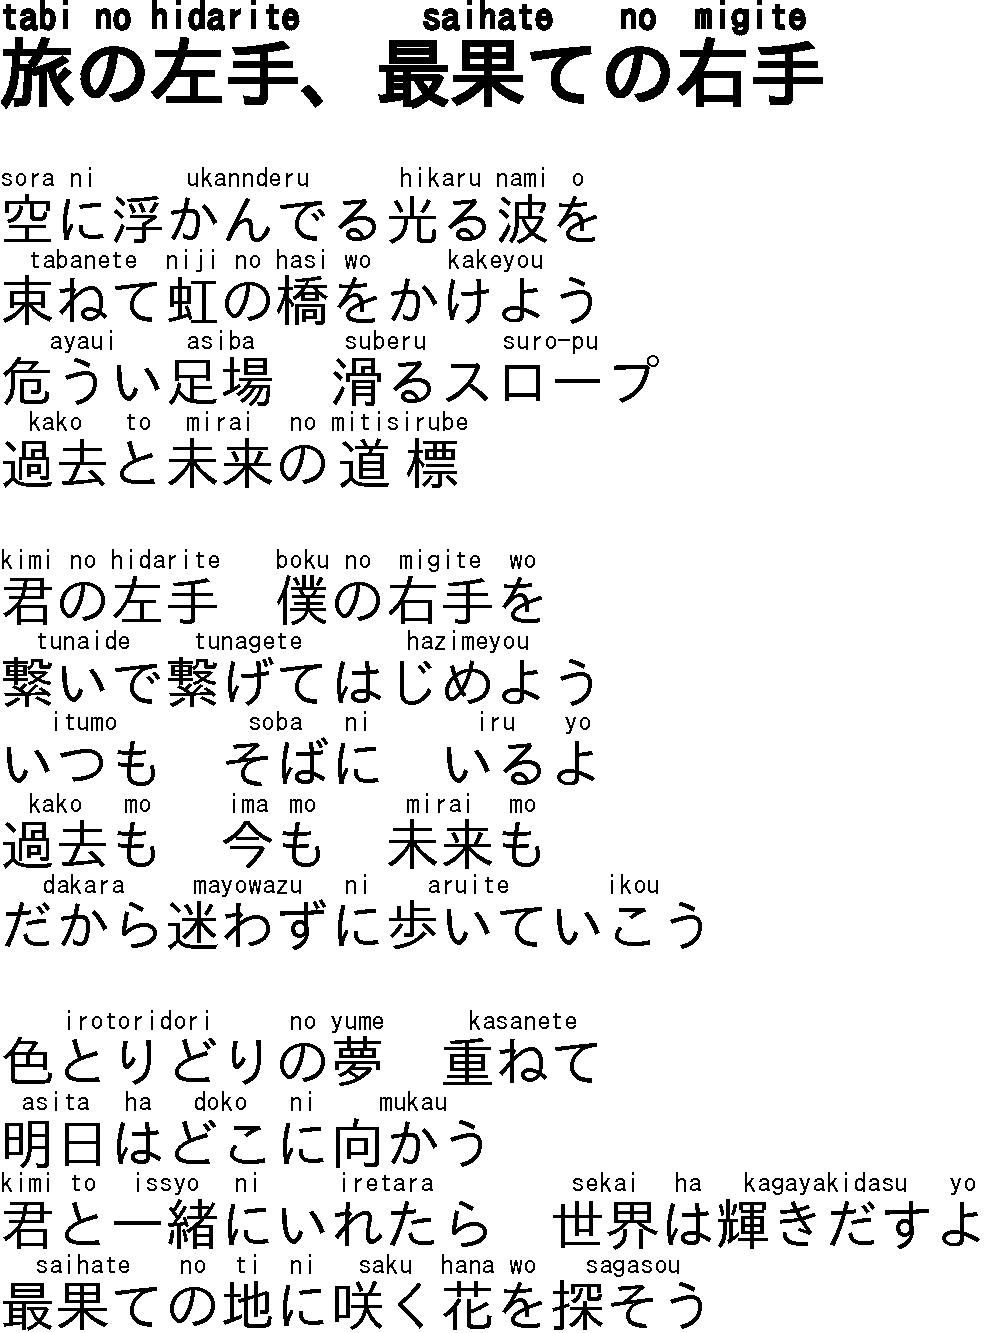
\includegraphics{../images/tabinohidaritesaihatenomigite}
\clearpage
\subsection{Made in Abyss}
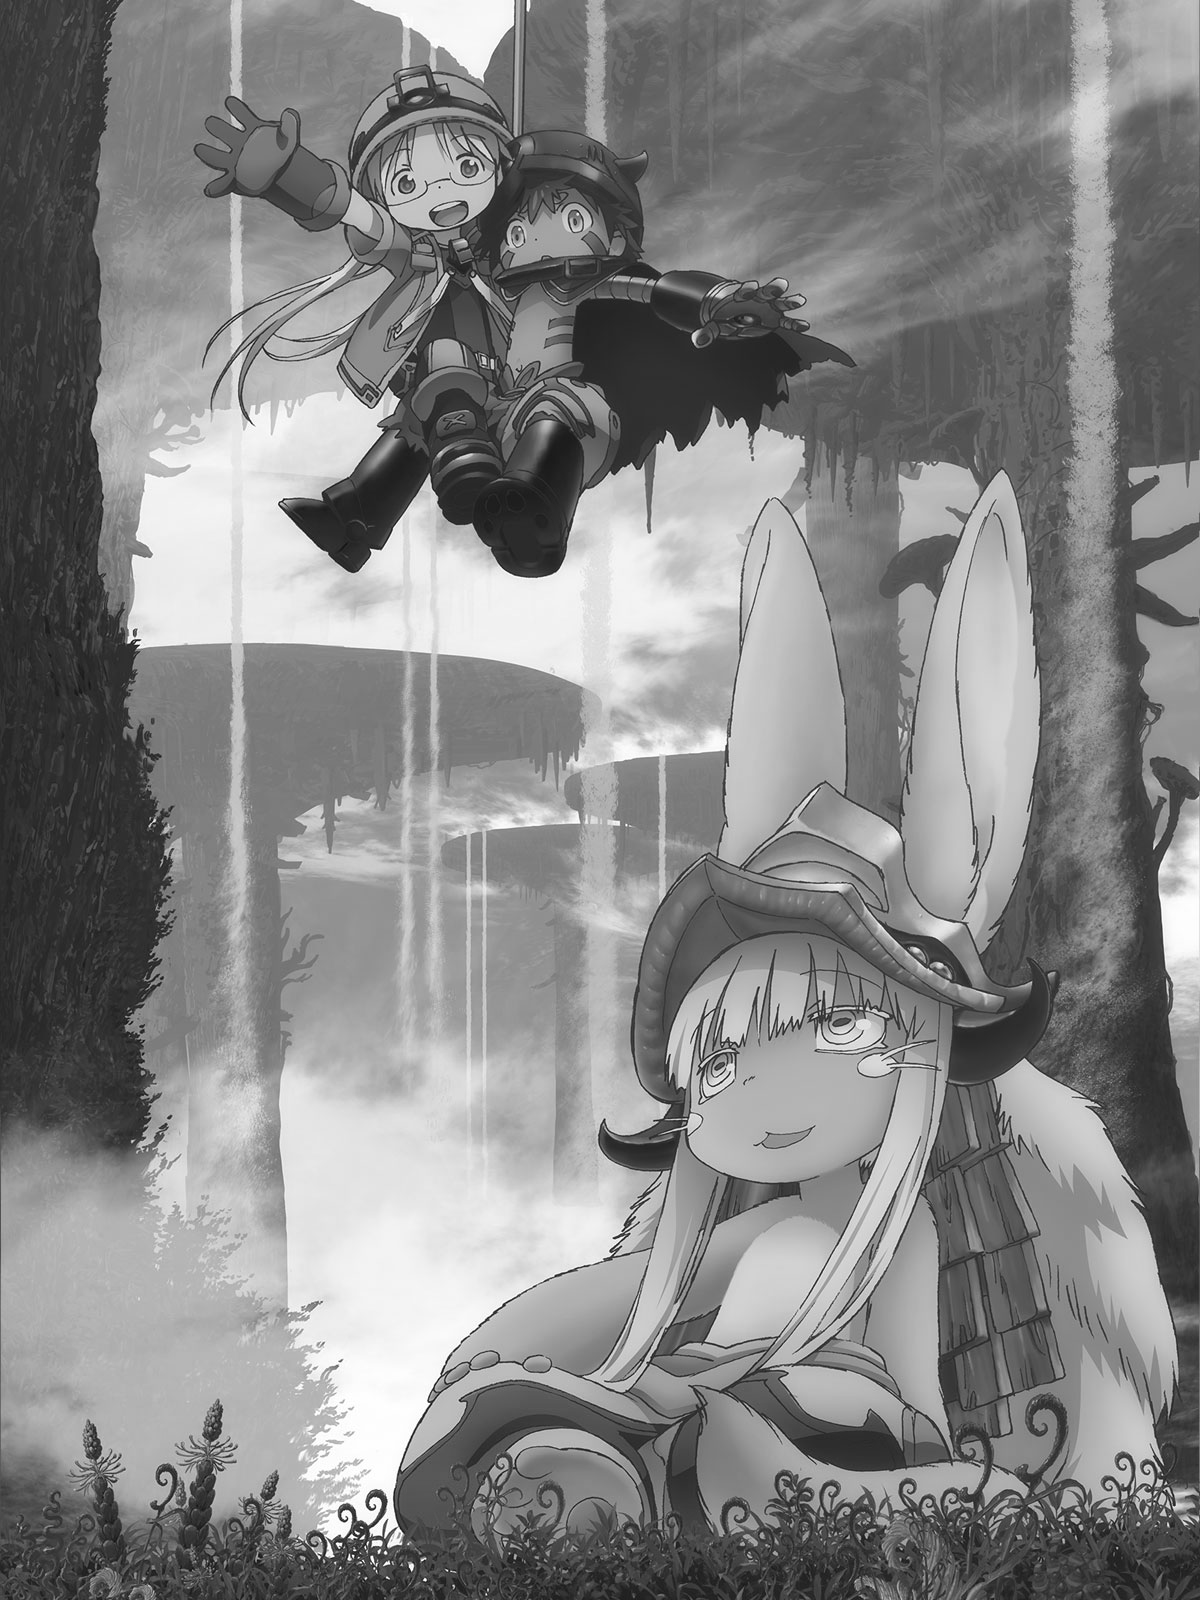
\includegraphics[width=7in]{../images/miabyss}
\end{document}
